% For LaTeX-Box: root = stat305-pexam1.Rnw
\documentclass[addpoints]{examsetup}\usepackage[]{graphicx}\usepackage[]{color}
%% maxwidth is the original width if it is less than linewidth
%% otherwise use linewidth (to make sure the graphics do not exceed the margin)
\makeatletter
\def\maxwidth{ %
  \ifdim\Gin@nat@width>\linewidth
    \linewidth
  \else
    \Gin@nat@width
  \fi
}
\makeatother

\definecolor{fgcolor}{rgb}{0.345, 0.345, 0.345}
\newcommand{\hlnum}[1]{\textcolor[rgb]{0.686,0.059,0.569}{#1}}%
\newcommand{\hlstr}[1]{\textcolor[rgb]{0.192,0.494,0.8}{#1}}%
\newcommand{\hlcom}[1]{\textcolor[rgb]{0.678,0.584,0.686}{\textit{#1}}}%
\newcommand{\hlopt}[1]{\textcolor[rgb]{0,0,0}{#1}}%
\newcommand{\hlstd}[1]{\textcolor[rgb]{0.345,0.345,0.345}{#1}}%
\newcommand{\hlkwa}[1]{\textcolor[rgb]{0.161,0.373,0.58}{\textbf{#1}}}%
\newcommand{\hlkwb}[1]{\textcolor[rgb]{0.69,0.353,0.396}{#1}}%
\newcommand{\hlkwc}[1]{\textcolor[rgb]{0.333,0.667,0.333}{#1}}%
\newcommand{\hlkwd}[1]{\textcolor[rgb]{0.737,0.353,0.396}{\textbf{#1}}}%
\let\hlipl\hlkwb

\usepackage{framed}
\makeatletter
\newenvironment{kframe}{%
 \def\at@end@of@kframe{}%
 \ifinner\ifhmode%
  \def\at@end@of@kframe{\end{minipage}}%
  \begin{minipage}{\columnwidth}%
 \fi\fi%
 \def\FrameCommand##1{\hskip\@totalleftmargin \hskip-\fboxsep
 \colorbox{shadecolor}{##1}\hskip-\fboxsep
     % There is no \\@totalrightmargin, so:
     \hskip-\linewidth \hskip-\@totalleftmargin \hskip\columnwidth}%
 \MakeFramed {\advance\hsize-\width
   \@totalleftmargin\z@ \linewidth\hsize
   \@setminipage}}%
 {\par\unskip\endMakeFramed%
 \at@end@of@kframe}
\makeatother

\definecolor{shadecolor}{rgb}{.97, .97, .97}
\definecolor{messagecolor}{rgb}{0, 0, 0}
\definecolor{warningcolor}{rgb}{1, 0, 1}
\definecolor{errorcolor}{rgb}{1, 0, 0}
\newenvironment{knitrout}{}{} % an empty environment to be redefined in TeX

\usepackage{alltt}

\usepackage{etoolbox}
\usepackage{tikz,pgfplots}

%% For LaTeX-Box: root = stat105_exam1_info.tex 
%%%%%%%%%%%%%%%%%%%%%%%%%%%%%%%%%%%%%%%%%%%%%%%%%%%%%%%%%%%%%%%%%%%%%%%%%%%%%%%%
%  File Name: stat105_exam1_info.tex
%  Purpose:
%
%  Creation Date: 24-09-2015
%  Last Modified: Thu Sep 24 13:51:36 2015
%  Created By:
%%%%%%%%%%%%%%%%%%%%%%%%%%%%%%%%%%%%%%%%%%%%%%%%%%%%%%%%%%%%%%%%%%%%%%%%%%%%%%%%
\newcommand{\course}[1]{\ifstrempty{#1}{STAT 105}{STAT 105, Section #1}}
\newcommand{\sectionNumber}{B}
\newcommand{\examDate}{October 1, 2015}
\newcommand{\semester}{FALL 2015}
\newcommand{\examNumber}{II}

\newcommand{\examTitle}{Exam \examNumber}

\runningheader{\course{\sectionNumber}}{Exam \examNumber}{\examDate}
\runningfooter{}{}{Page \thepage of \numpages}

\newcommand{\examCoverPage}{
   \begin{coverpages}
   \centering
   {\bfseries\scshape\Huge Exam I \par}
   \vspace{1cm}
   {\bfseries\scshape\LARGE \course{\sectionNumber} \par}
   {\bfseries\scshape\LARGE \semester \par}

   \vspace{2cm}

   \fbox{\fbox{\parbox{5.5in}{\centering 

      \vspace{.25cm} 
      
      {\bfseries\Large Instructions} \\

      \vspace{.5cm} 

      \begin{itemize}
         \item  The exam is scheduled for 80 minutes, from 8:00 to 9:20 AM. At 9:20 AM the exam will end.\\
         \item  A forumula sheet is attached to the end of the exam. Feel free to tear it off.\\
         \item  You may use a calculator during this exam.\\
         \item  Answer the questions in the space provided. If you run out of room, continue on the back of the page. \\
         \item  If you have any questions about, or need clarification on the meaning of an item on this exam, please ask your instructor. No other form of external help is permitted attempting to receive help or provide help to others will be considered cheating.\\
         \item  {\bfseries Do not cheat on this exam.} Academic integrity demands an honest and fair testing environment. Cheating will not be tolerated and will result in an immediate score of 0 on the exam and an incident report will be submitted to the dean's office.\\
      \end{itemize}

   }}}

   \vspace{2cm}

   \makebox[0.6\textwidth]{Name:\enspace\hrulefill}

   \vspace{1cm}

   \makebox[0.6\textwidth]{Student ID:\enspace\hrulefill}
   \end{coverpages}

}


\newcommand{\course}[1]{\ifstrempty{#1}{STAT 305}{STAT 305, Section #1}}
\newcommand{\sectionNumber}{D}
\newcommand{\examDate}{February 21, 2019}
\newcommand{\semester}{FALL 2019}
\newcommand{\examNumber}{I}
\IfFileExists{upquote.sty}{\usepackage{upquote}}{}
\begin{document}

%-- : R code (Code in Document)



\examCoverPage

\begin{questions}


\question[2] 
Circle the \textbf{bold face} term that makes the following statement true: \\

A measurement device that reports the measurements which are close to each other when repeatedly measuring the same thing is (\textbf{precise} or \textbf{accurate}).
\vspace{1cm}

\question[2] 
When dealing with qualitative data, the best way to describe the common value is using the (\textbf{mode} or \textbf{mean} or \textbf{median}).
\vspace{1cm}


\question
%-- : R code (Code in Document)


A sample of size 5 was drawn from a population and the resulting observations are reported below. 
\begin{center}
110, 100, 105, 103, 105, 115
\end{center}
Using these observed values, report the following:
\vspace{1cm}

\begin{parts}

   \part[2] the mean  
   \vspace{1.5cm}

   \part[2] the mode
   \vspace{1.5cm}

   \part[2] the median 
   \vspace{1.5cm}

   \part[2] the variance 
   \vspace{1.5cm}

   \part[2] the standard deviation 
   \vspace{1.5cm}

   \part[2] the value of $Q(.75)$
   \vspace{1.5cm}

   \part[2] the interquartile range
   \vspace{1.5cm}

\end{parts}


\question

In the field of psychology, the Dunning–Kruger effect is a cognitive bias in which people of low ability overestimate their ability and students with high ability underestimate their ability.
In order to study this phenomenon, a team of psychologists at Iowa State asked students from the College of Liberal Arts and Sciences to estimate the score they would receive on a standardized grammar test (as a percentage from 0 to 100).
They recorded the student's sex, age, and major. 
The students were then given the standardized grammar test with 50 questions and the number of correct answers was recorded.

\begin{parts}
   \part[2] Is this an experiment or an observational study?
   \vspace{2cm}
   
   \part[2] What is the population under study?
   \vspace{2cm}

   \part For each of the following variables, 

   \begin{itemize}

      \item Identify whether it is qualitative or quantitative variable, and 

      \item If it is qualitative, provide the values it can take (if there are more than three, list at least three).

      \item If it is quantitative, is it continuous or discrete?

   \end{itemize}

   \begin{subparts}

      \subpart the number of questions the student answered correctly on the standardized test.

      \vspace{2cm}

      \subpart The score the student predicted they would recieve on the standardized test.

      \vspace{2cm}

      \subpart The student's sex.

      \vspace{2cm}

      \subpart The student's age.

      \vspace{2cm}

      \subpart The student's major.

   \end{subparts}

\end{parts}
\pagebreak


\question \textbf{Twin Cinema}

A professor of theoretical sociology is convinced that horror movies contribute to anxiety.
In order to test his hypothesis, the professor arranged to have to students in his class go to a movie showing on campus for extra credit. 
However, he randomly told half the students to see a movie in one location (location A) showing a scary movie!
The other half of his students, he sent to a second location (location B) showing a romantic comedy.
In order to fund this experiment throught the National Institute of Health, the professor added a nutrition component: in order to examine the effect of diet on anxiety, he gave the students a voucher which could be redeemed for either a high caffeine soda, a tub of popcorn, or a candy snack.
At the end of the movies, he recorded which movie the student had seen, which snack they had chosen, and then gave the student a questionairre that scored the student as having low, medium, or high anxiety.

\begin{parts}
   \part[2] Is this an experiment or an observational study? Explain.

  \vspace{2cm}

   \part Identify the following (if there was not one, simply put "not used").

  \vspace{1cm}

   \begin{subparts}
      \subpart[2] Response variable(s):

      \vspace{2cm}

      \subpart[2] Experimental variable(s):

      \vspace{2cm}

      \subpart[2] Blocking variable(s):

      \vspace{2cm}

   \end{subparts}

   \part[2] Was replication used in this experiment? If so, where was it applied? If not, how could we have applied it?

  \vspace{2cm}

\end{parts}
\pagebreak


\question \textbf{From Blown Speakers}

%-- Problem setup code


In car audio speakers, large changes in the intensity of sound produced by the speaker may cause a speaker component known as a cone to vibrate non-uniformly. 
The non-uniform vibrations of the cone cause the cone to add stress to the materials surrounding the cone. 
The damage to the surrounding materials results in the sound produced by the speakers becoming crackly - a state in which the speaker is "blown out".

Audio engineers working on ways to stabilize the cone during large changes in intensity are reviewing data that a 
new "smart" audio system collects and reports information when a blown speaker is detected. 
The following is a list of the \textbf{change in intensity} (as measured in decibels) from the first 35 audio systems that sent a blown speaker report.

%-- : R code (Code in Document)
\begin{knitrout}
\definecolor{shadecolor}{rgb}{0.969, 0.969, 0.969}\color{fgcolor}\begin{kframe}
\begin{verbatim}
 [1] 25.4 22.2 13.7 18.6 15.5 38.4 23.3 14.9 18.7 25.5 22.6 25.8 37.5 22.0
[15] 23.2 20.4 22.6 16.8 17.1 23.5 21.0 23.7 24.8 14.3 20.3 26.7 20.8 38.2
[29] 15.3 27.9  3.8  2.7 16.5 23.5 15.4
\end{verbatim}
\end{kframe}
\end{knitrout}

In this case, the range is 35.7, Q1 is 16.575, Q2 is 22, and the IQR is 2.525.

\begin{parts}
  \part[5] Fill in the values for the 5-number summary table: \\
  \begin{table}[h!]
     \centering
     \begin{tabular}{|l|p{3cm}|p{3cm}|p{3cm}|p{4cm}|}
     \hline
     \textbf{Minimum} & \textbf{First Quartile} & \textbf{Median} & \textbf{Third Quartile} & \textbf{Maximum} \\ \hline \hline
                      &                         &                 &                         &                  \\
                      &                         &                 &                         &                  \\
                      &                         &                 &                         &                  \\
     \hline
     \end{tabular}
  \end{table}
  
  \part[10] Complete the following frequency table using 8 equal length intervals for the value range (it should include all the data): \\

  \begin{table}[h!]
     \centering
     \begin{tabular}{|l|p{3cm}|p{3cm}|p{4cm}|}
     \hline
                          & \textbf{Frequency} & \textbf{Relative}  & \textbf{Cumulative}  \\
     \textbf{Value Range} &                    & \textbf{Frequency} & \textbf{Relative Frequency} \\\hline \hline
     &  &  &  \\
     &  &  &  \\
     \hline
     &  &  &  \\
     &  &  &  \\
     \hline
     &  &  &  \\
     &  &  &  \\
     \hline
     &  &  &  \\
     &  &  &  \\
     \hline
     &  &  &  \\
     &  &  &  \\
     \hline
     &  &  &  \\
     &  &  &  \\
     \hline
     &  &  &  \\
     &  &  &  \\
     \hline
     &  &  &  \\
     &  &  &  \\
     \hline
     \end{tabular}
  \end{table}

  \pagebreak

  \part[5] Create a \textbf{frequency histogram} to summarize the data. Carefully label the axes.

  \vspace{4cm}

  \part[10] Create a box plot to summarize the data. Carefully label the axes.

  \vspace{4cm}

  \part[4] Are there any unusually observations? If so what were the speeds for those observations?

  \vspace{3cm}

  \part[10] The engineers also get information about how far the base of the cone was displaced during the blowout. Here are some of the displacements:

%-- : R code (Code in Document)


\begin{center}
   0, 0.3, 0.4, 0.6, 0.7, 0.7, 0.8, 1, 1.3, 3.5
\end{center}

Create a theoretical Q-Q plot using the following quantiles from the normal distribution as the theoretical quantiles. Carefully label your axes.
What does this graph tell us about the upload speeds?

\begin{table}[h!]
   \centering
   \begin{tabular}{ccccccccccc}
             & 1 & 2 & 3 & 4 & 5 & 6 & 7 & 8 & 9 & 10 \\ \hline
      $p$    & 0.05 & 0.15 & 0.25 & 0.35 & 0.45 & 0.55 & 0.65 & 0.75  & 0.85 & 0.95 \\
      $Q(p)$ & -1.64 & -1.04 & -0.67 & -0.39 & -0.13 & 0.13 & 0.39 & 0.67 & 1.04 & 1.64 \\ \hline
   \end{tabular}
\end{table}


\end{parts}
\pagebreak


\question \textbf{Champions Red Wine}
%-- : R code (Code in Document)


Oenophiles, or connoisseurs of fine wines, have been benefitted by sort of open information sharing we have in the days of online auctions. 
By monitoring the prices for which sought after bottles actually sell for, wine enthusiasts are able to both determine whether or not they are getting a fair price and whether or not they might make a nice profit by selling off a few of the bottles they have in storage.
Before this era of easy and free data though, there was one source of information that stood above all the others: \textit{Le Champions de vin rouge}, a guide to the world of fine wines published in 1997.
While the information contained it in is largely still relevant in general, the price index has become somewhat outdated.

Or has it? 
Is it possible that the prices from the guide in 1997 could help us understand the market today?
A certain statistician decided to do a deep analysis of the relationship between the cost of wine bottles in the 1997 book and the actual prices the same bottles fetched on open auction sites recently. 
The dataset he created consists of the last 500 bottles with publically available auction prices that were also listed in \textit{Le Champions de vin rouge} price index.

\begin{center}
\begin{knitrout}
\definecolor{shadecolor}{rgb}{0.969, 0.969, 0.969}\color{fgcolor}
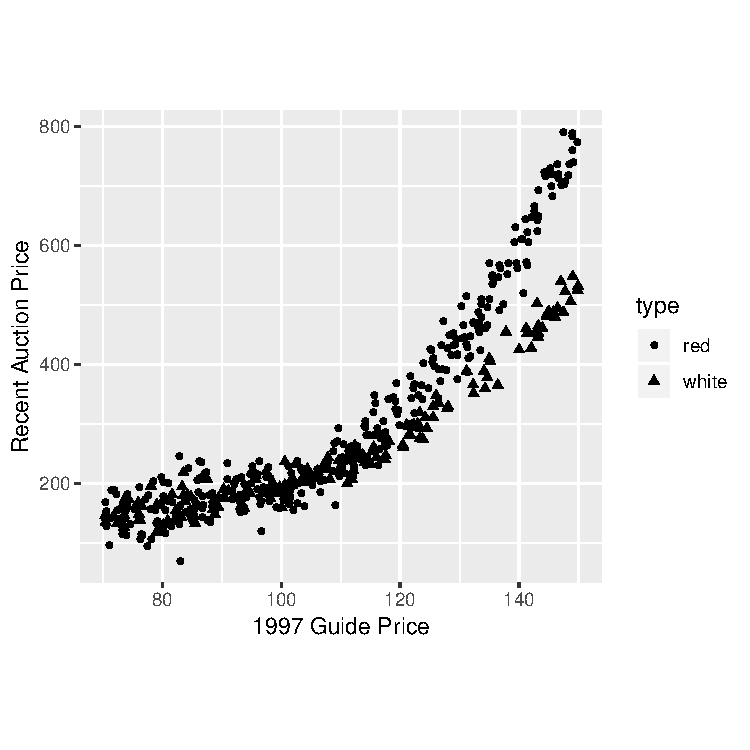
\includegraphics[width=.5\linewidth]{figure/unnamed-chunk-13-1} 

\end{knitrout}
\end{center}

Here are some summaries of the dataset with the 1997 Guide Price as $x$ and the Recent Auction Price as $y$.

$$
\sum_{i=1}^{500} x_i = 54348 \hspace{3cm} \sum_{i=1}^{500} x_i^2 = 6164828 \\
$$

$$
\sum_{i=1}^{500} y_i = 146782 \hspace{3cm} \sum_{i=1}^{500} y_i^2 = 55928348 \\
$$

$$
\sum_{i=1}^{500} x_i y_i = 17573001
$$

\pagebreak

\begin{parts}
   \part Using the summaries, fit a linear relationship between \textbf{1997 Guide Price} (x) and \textbf{Recent Auction Price} (y). 
   \begin{subparts}
      \subpart[5] Write the equation of the fitted linear relationship. 
      \vspace{4cm}
      \subpart[5] Find and interpret the value of $R^2$ for the fitted linear relationship.
      \vspace{3cm}
      \subpart[5] Using the fitted line, provide a predicted Recent Auction Price when the 1997 Guide Price was \$120.
      \vspace{3cm}
      \subpart[5] Sketch what you believe the plot of residuals vs 1997 Guide Price would look like. Why would this be a problem?
      \vspace{3cm}
      \subpart[3] The points in the plot have different shapes based on whether the wine is "Red" or "White." Is there a reason to believe that white wines and red wines should not be modeled together? Explain why.
      \vspace{2cm}
   \end{subparts}

\pagebreak

   \part 
   The JMP output below comes from fitting a quadratic model using $x$ and $x^2$ for \textit{Red Wine Only} (left) and \textit{White Wine Only} (right).

  \begin{figure}[!h]
  \begin{subfigure}
  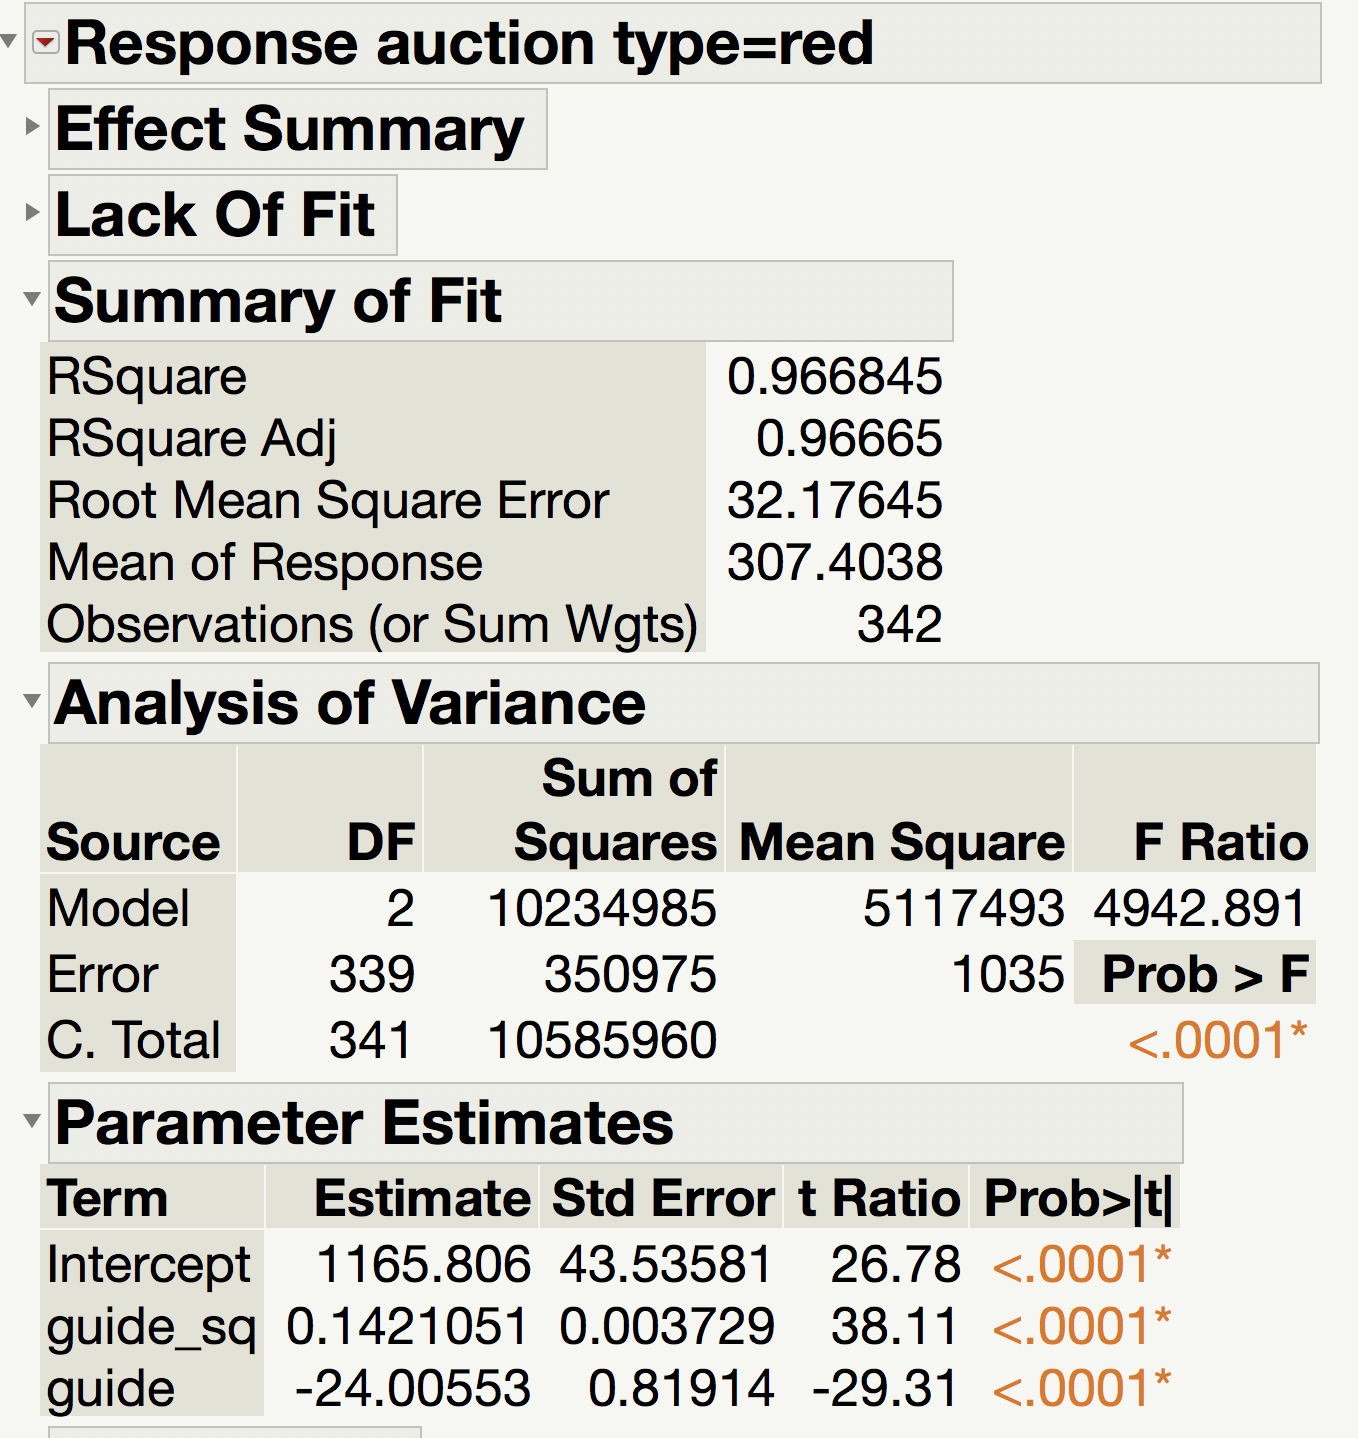
\includegraphics[scale=.3]{figure/red-wine-quadratic}
  \end{subfigure}
  \begin{subfigure}
  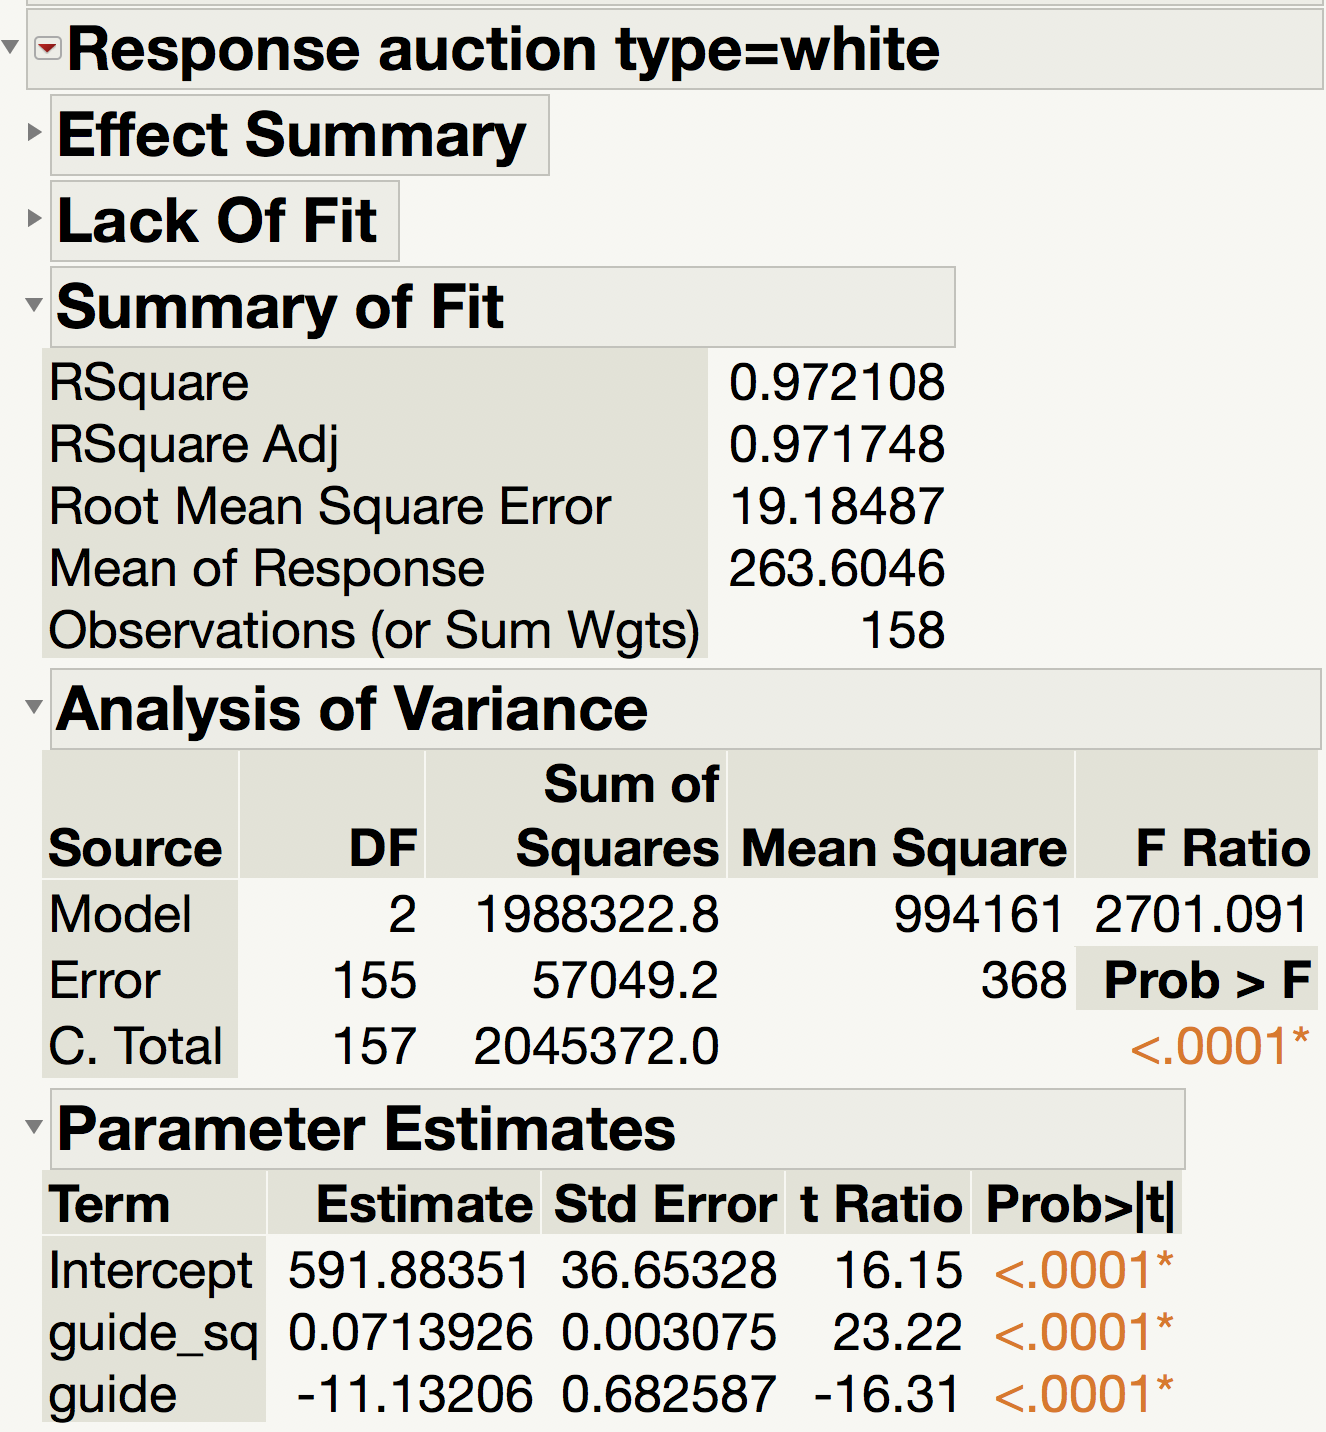
\includegraphics[scale=.3]{figure/white-wine-quadratic}
  \end{subfigure}
  \end{figure}

   \begin{subparts}
      \subpart[5] Write the equation of the fitted quadratic relationship \textit{for Red Wines}. 
      \vspace{2cm}
      \subpart[5] Write the equation of the fitted quadratic relationship \textit{for White Wines}. 
      \vspace{2cm}
      \subpart[5] Interpret the value of $R^2$ for the two fitted quadratic relationships.
      \vspace{2cm}
      \subpart[5] Using the fitted quadratic relationship, provide a predicted value of Recent Auction Price for a red wine with 1997 Guide Price of \$120.
   \end{subparts}
\end{parts}



\end{questions}

\end{document}
